\documentclass{article}
\usepackage{graphicx}
\usepackage[margin=1.5cm]{geometry}
\usepackage{amsmath}

\begin{document}

\title{Wednesday Reading Assessment: Unit 0, Voltage}
\author{Prof. Jordan C. Hanson}

\maketitle

\section{Memory Bank}

\begin{itemize}
\item $PE = q V$ ... Relationship between potential energy, charge, and voltage.
\item $PE = m g h$ ... Gravitational potential energy.
\item $KE = \frac{1}{2}m v^2$ ... Definition of kinetic energy.
\end{itemize}

\section{Electric Potential and Potential Energy}

\begin{enumerate}
\begin{figure}[ht]
\centering
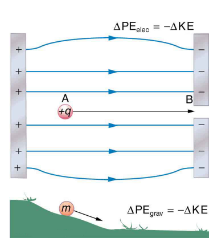
\includegraphics[width=0.22\textwidth]{hill.png}
\caption{\label{fig:hill} The relationship between potential energy and voltage.}
\end{figure}
\item Consider Fig. \ref{fig:hill}.  Suppose the mass $m$ rolls down a hill from a height of 30 meters.  In the absense of \textit{friction}, what will be the final speed of the object? \\ \vspace{1cm}
\item Consider Fig. \ref{fig:hill}.  Suppose the charge is $q = 1 \mu$C, and the voltage is 12 V.  (a) What is the potential energy before the charge is released? (b) If the charge has a mass of $10^{-6}$ kg, what will the final speed be after the charge is released? \\ \vspace{1.5cm}
\item What voltage would be required to \textit{stop} the charge from moving?
\begin{itemize}
\item A: 6 V
\item B: 10 V
\item C: 12 V
\item D: -12 V
\end{itemize}
\end{enumerate}

\end{document}
